\newpage
\section{Analisi della Homepage}

\subsection{Le 5+1 W}
Il modo più formale di analizzare l'impatto che una pagina web ha su un utente è rispondere alle famose \textit{6Ws del giornalismo}, le quali sono:
\begin{itemize}
\item Where?
\item Who?
\item Why?
\item What?
\item When?
\item How?
\end{itemize}

\subsubsection{Where?}
\textsc{Where} corrisponde alla domanda \textsc{dove mi trovo?}. Un utente qualsiasi che visita la pagina per la prima volta si trova davanti a questa schermata.

\vspace{30pt}
\begin{figure}[htbp]
\begin{center}
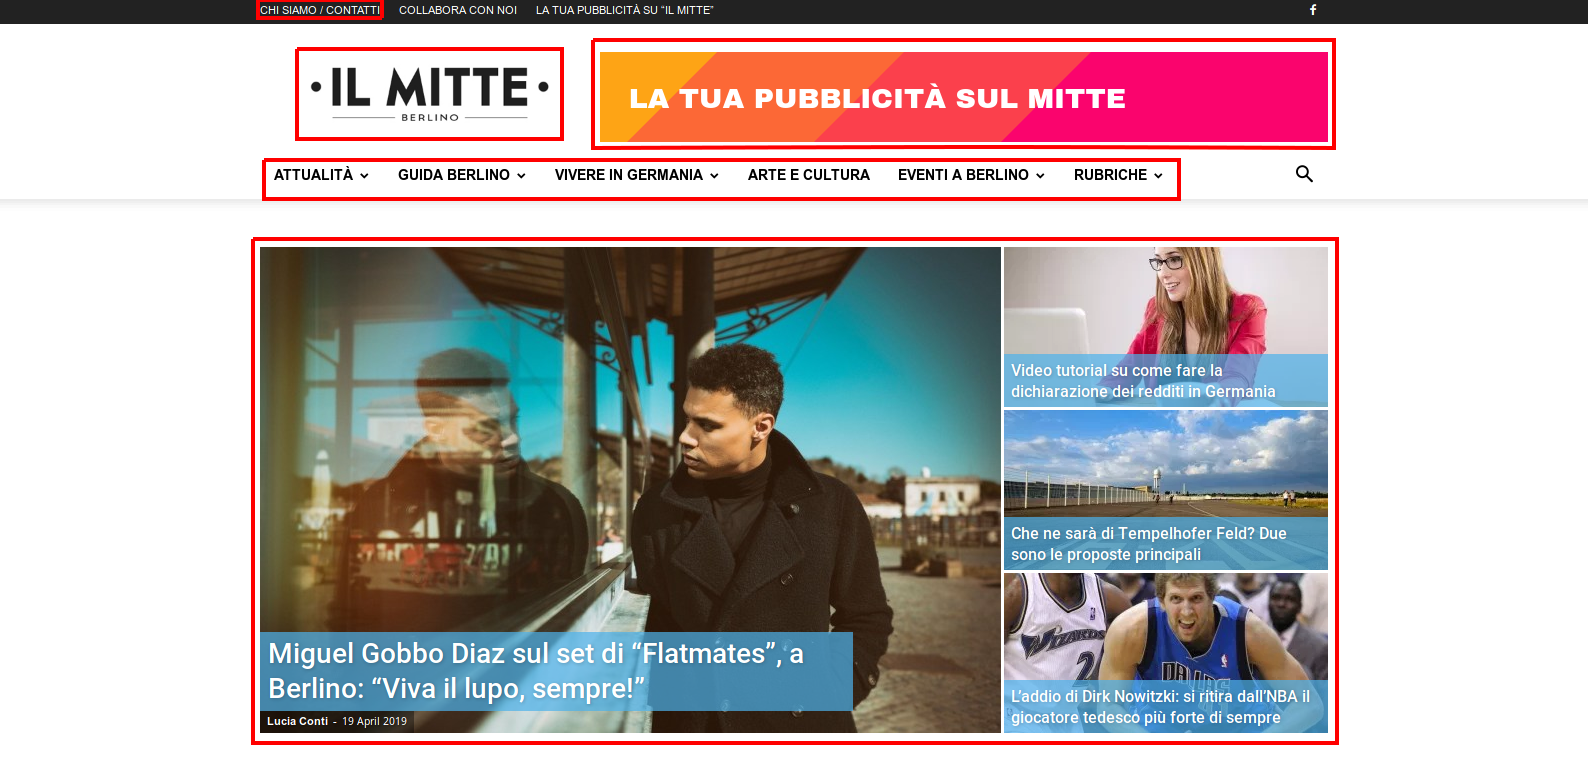
\includegraphics[width=35em]{img/home1}
\caption{Prima schermata Homepage}
\end{center}
\end{figure}
\vspace{30pt}

La prima area su cui si focalizza l'utente è sicuramente l'\textit{header}. \\
In questa pagina il primo sguardo si ferma sul logo, e successivamente sul banner pubblicitario (al momento ancora inutilizzato); il logo informa molto chiaramente sul nome del sito in cui ci si trova, ma non fornisce una spiegazione esaustiva di cosa sia e a cosa serva il sito. \\
L'attenzione si sposta poi sul menù, che fornisce parzialmente del contesto: le voci, \texttt{Attualità}, \texttt{Guida Berlino}, \texttt{Vivere in Germania}, \texttt{Arte e cultura}, \texttt{Eventi a Berlino} e \texttt{Rubriche}, danno probabilmente l'idea che questo sia il sito di un giornale online. \\
Successivamente, l'attenzione si sposta sull'immagine più grande, che corrisponde all'anteprima dell'ultimo articolo, e a seguire i tre articoli più recenti dopo l'ultimo, ordinati in modo decrescente per data. \\
Procedendo con lo scroll della pagina, nella prima schermata si possono leggere altre \textit{News}; nella seconda e nella terza schermata si visualizzano due griglie 3x3 composte dalle anteprime degli articoli appartenenti alle sezioni \texttt{Guida Berlino} e \texttt{Vivere in Germania} rispettivamente. \\

\vspace{30pt}
\begin{figure}[htbp]
\begin{center}
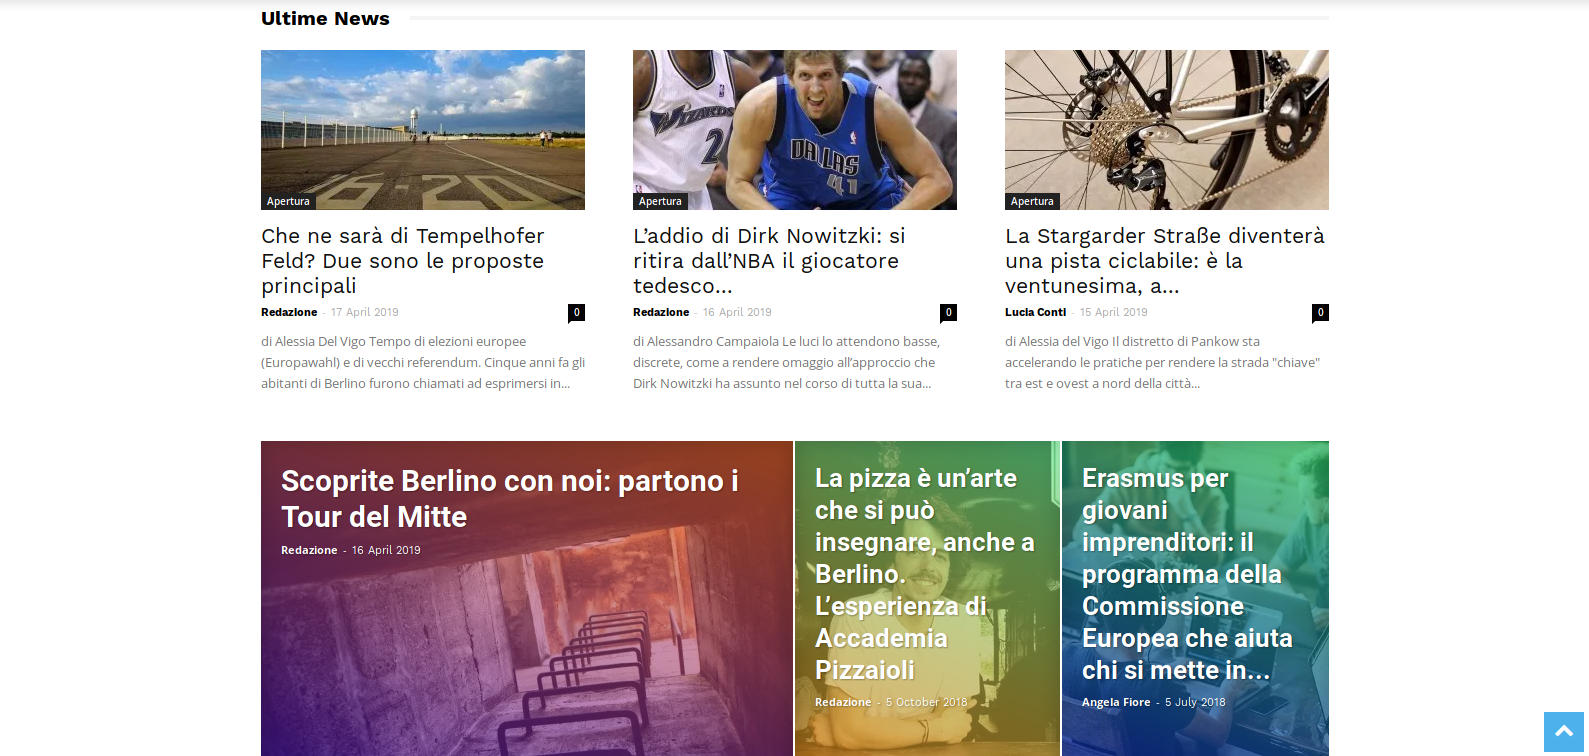
\includegraphics[width=35em]{img/home2}
\caption{Seconda schermata Homepage - Ultime News}
\end{center}
\end{figure}
\vspace{30pt}

\begin{figure}[htbp]
\begin{center}
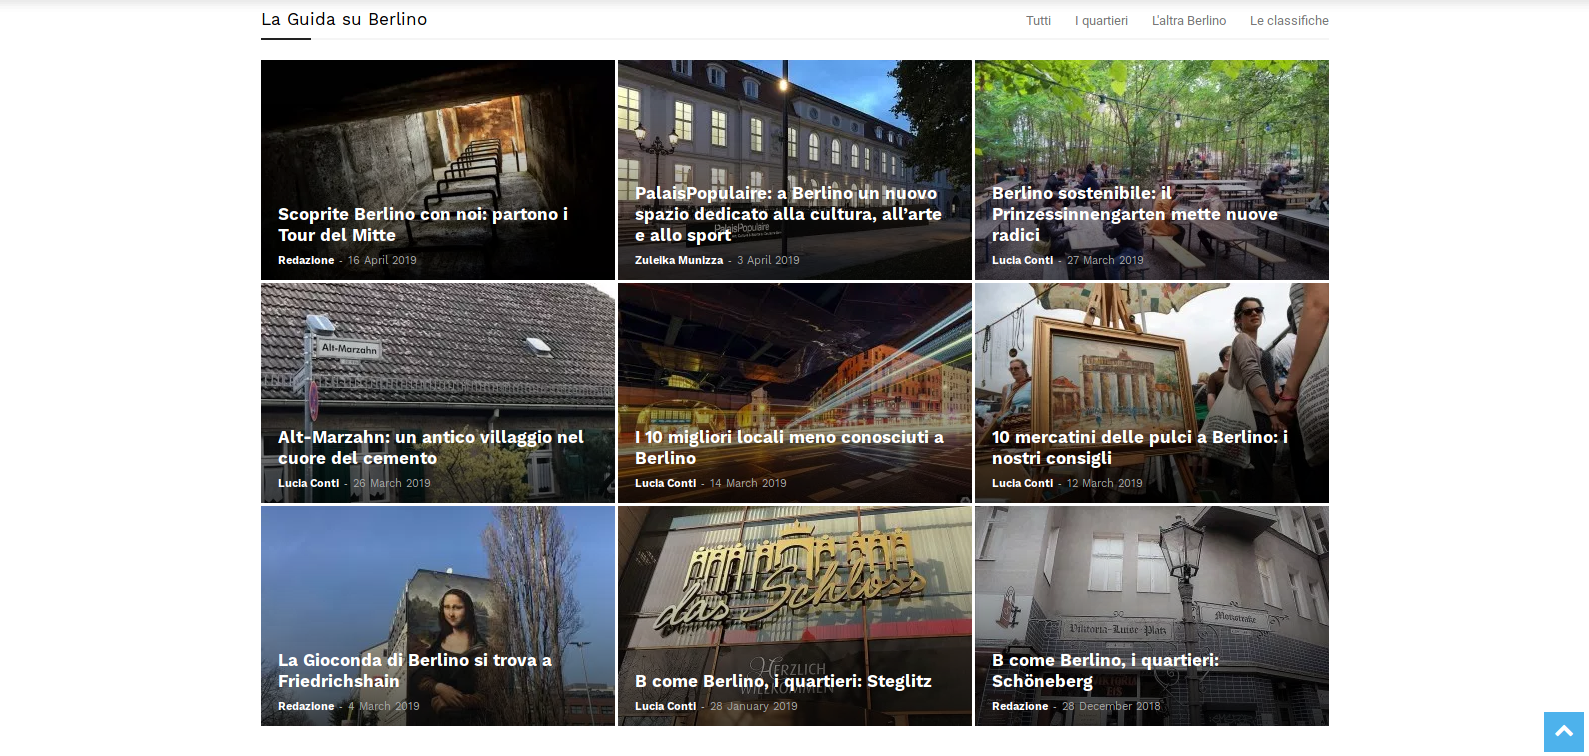
\includegraphics[width=35em]{img/home3}
\caption{Terza schermata Homepage - Griglia 3x3 esplicativa}
\end{center}
\end{figure}
\vspace{30pt}


Al quarto scroll si arriva alle anteprime della sezione \texttt{Arte e cultura}, ma lo stile ora è diverso: gli articoli sono visualizzati in forma di lista, e alla destra di essi si configura la sezione \texttt{Classifiche}. \\
Tutte queste informazioni probabilmente forniscono all'utente l'informazione cercata: il sito è un giornale online. Come lo faccia, però, è discutibile: lo stile è confusionario e disomogeneo, e rischia di creare confusione nella \textbf{mappa mentale} che l'utente si crea del sito. \\

\vspace{30pt}
\begin{figure}[htbp]
\begin{center}
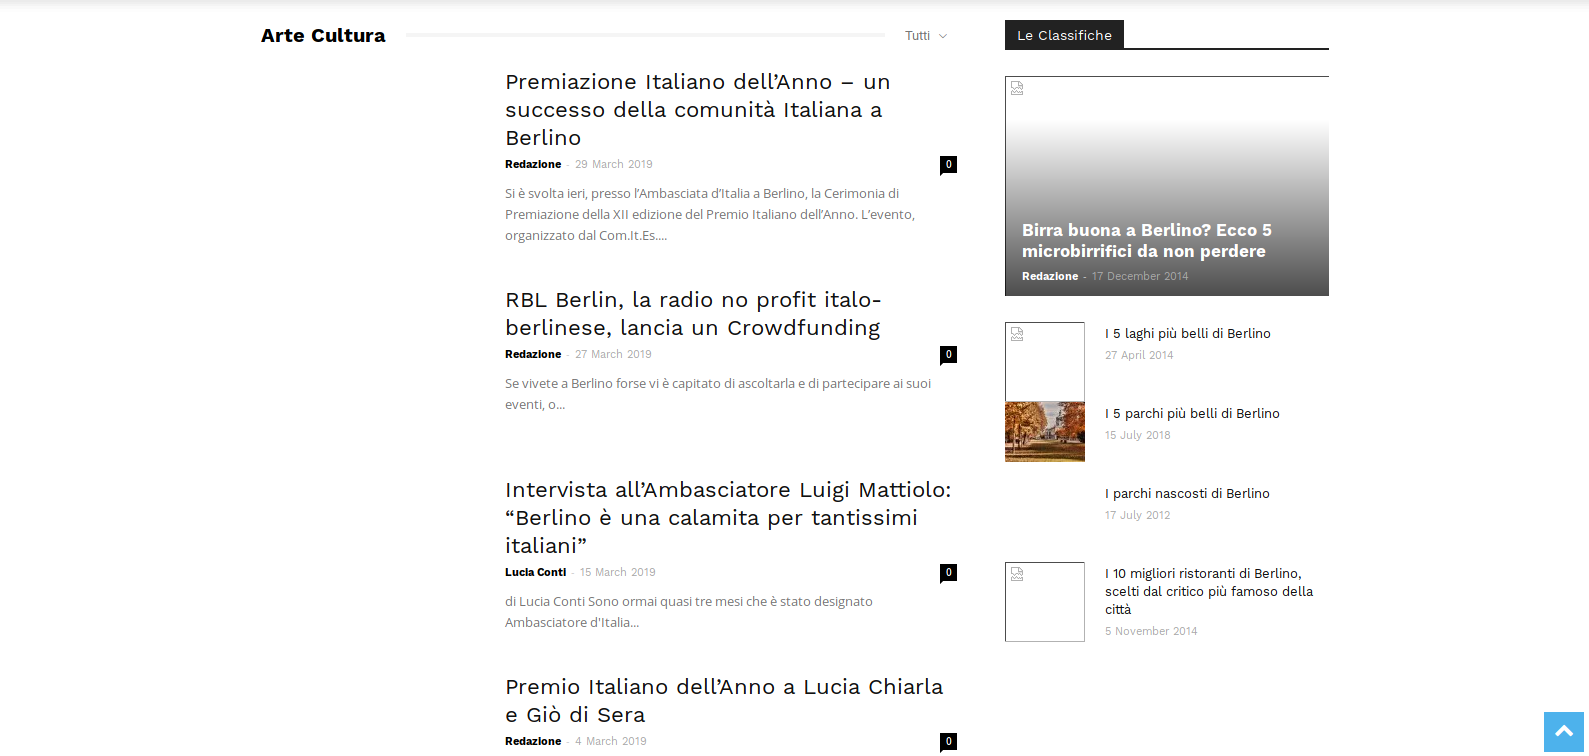
\includegraphics[width=35em]{img/home4}
\caption{Quarta schermata Homepage - Struttura disomogenea. Si possono notare anche le immagini corrotte, che contribuiscono alla sensazione di disordine.}
\end{center}
\end{figure}
\vspace{30pt}

\newpage

\subsubsection{Who?}
\textsc{Who} corrisponde alla domanda \textsc{chi c'è dietro al sito?}. Questa informazione ci è fornita solo dal logo. Per avere una risposta definitiva su chi sia dietro al sito, l'utente sarà costretto a cliccare su \texttt{Chi siamo/contatti}, nella zona più in alto a sinistra della pagina. Sebbene la pagina risponda alle domande poste dall'utente, egli sarà stato costretto a cliccare su un link, che poteva però non dare l'informazione ricercata; ecco quindi un primo \textbf{gambling click} che rischia di rovinare l'esperienza e far scappare l'utente.

\vspace{30pt}
\begin{figure}[htbp]
\begin{center}
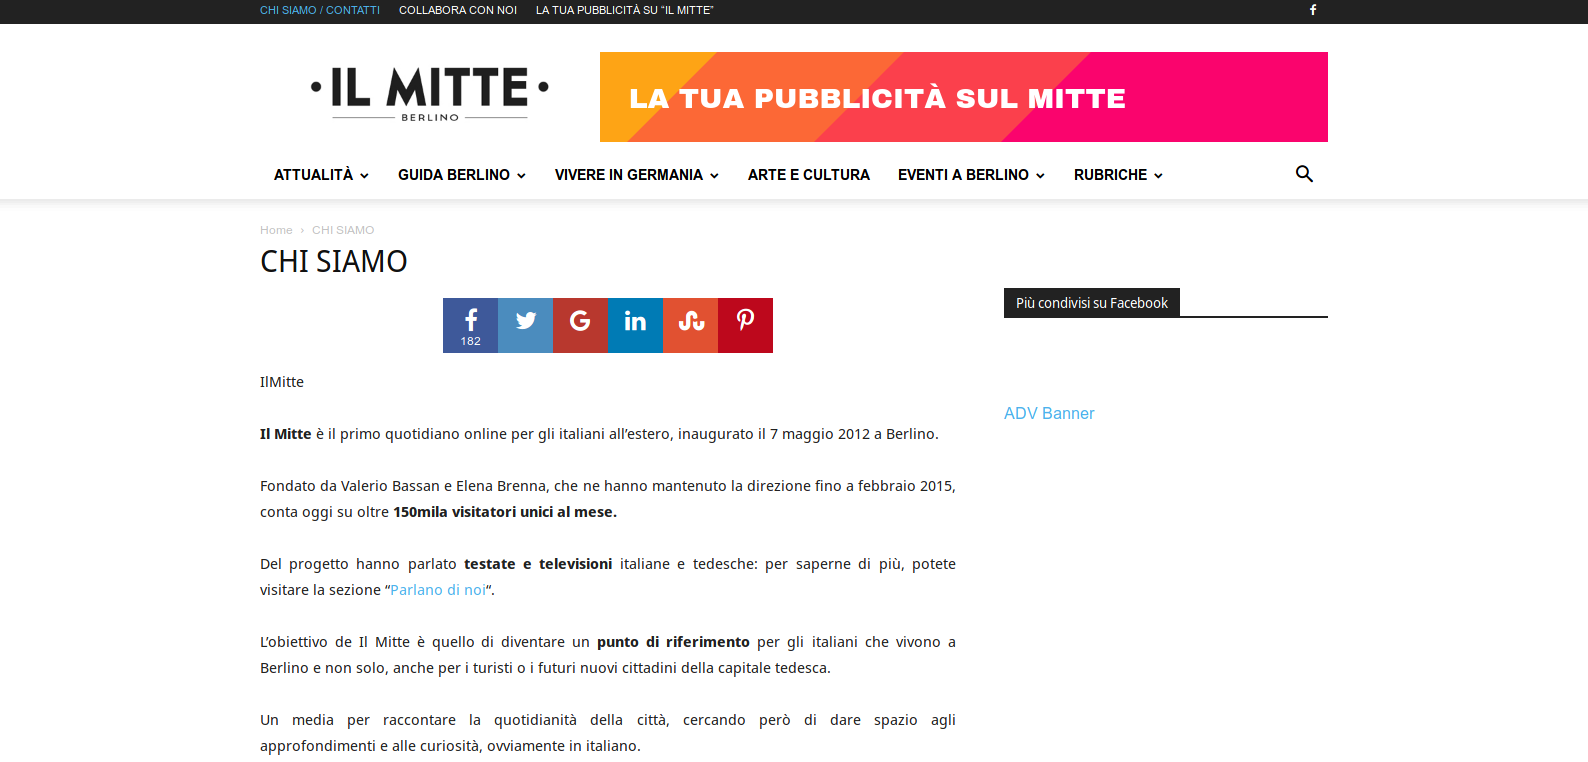
\includegraphics[width=35em]{img/chisiamo}
\caption{Sezione "Chi siamo/Contatti"}
\end{center}
\end{figure}
\vspace{30pt}

\subsubsection{What?}
\textsc{What} corrisponde alla domanda \textsc{cosa mi offre il sito?}. La risposta ci viene data immediatamente grazie al menù, che specifica le categorie di articoli che si possono trovare sul sito, e agli articoli in evidenza, che danno un chiaro esempio di titolo di un articolo. \\
Per quanto riguarda lo scroll, però, permangono i problemi esposti nella sezione \textsc{where}.

\subsubsection{Why?}
\textsc{Why} corrisponde alla domanda \textsc{perché sono qui?}. La risposta dovrebbe derivare direttamente dal \textsc{what} e dal \textsc{where}: il sito offre numerosi articoli e approfondimenti su Berlino e sulla vita in Germania. Se l'utente si trova qua, quindi, significa che è interessato a informarsi su questi argomenti.

\subsubsection{When?}
La risposta alla domanda \textsc{When}, \textsc{quali sono le ultime novità, cos'è cambiato?} è immediata e funzionale: gli ultimi articoli sono riportati in grande nella prima schermata della pagina, permettendo così un facile aggiornamento dell'utente.

\subsubsection{How?}
\textsc{How} corrisponde alla domanda \textsc{come arrivo a ciò che mi interessa?}. Gli strumenti di navigazione del sito sono due: il menù e la barra di ricerca; manca invece una mappa del sito.

\paragraph*{Menù}

Il menù si articola sull'header del sito. Lo stile è tutto sommato uniforme: passando con il dispositivo di puntamento sopra al nome della sezione questa viene sottolineata, e la tendina del menù scende portando con sé le anteprime di alcuni articoli. \\
Nei casi di \texttt{Guida Berlino}, \texttt{Eventi a Berlino} e \texttt{Rubriche} sono presenti anche delle sottosezioni, le quali fanno comparire a loro volta altri articoli con la sovrapposizione del mouse. \\
La sezione \texttt{Arte e cultura} non porta a nessun sottomenù, e questo potrebbe portare a una sorta di aspettativa tradita per l'utente; nonostante questo, però, le altre voci possiedono una freccia puntata verso il basso a indicare che sono presenti più voci, e quest'interfaccia è tutto sommato intuitiva. \\
Il problema principale del menù è la mancanza di \textbf{fault tolerance}: uscendo con il puntatore anche di un pixel, infatti, il menù scompare immediatamente. Questo provoca fastidio nell'utente, poiché molto scomodo. \\
Un altro problema consiste nel fatto che il menù scompaia con lo scroll. Sebbene un minimo scroll verso l'alto da qualsiasi parte della pagina lo faccia ricomparire, è comunque una scomodità che si poteva evitare.

\vspace{30pt}
\begin{figure}[htbp]
\begin{center}
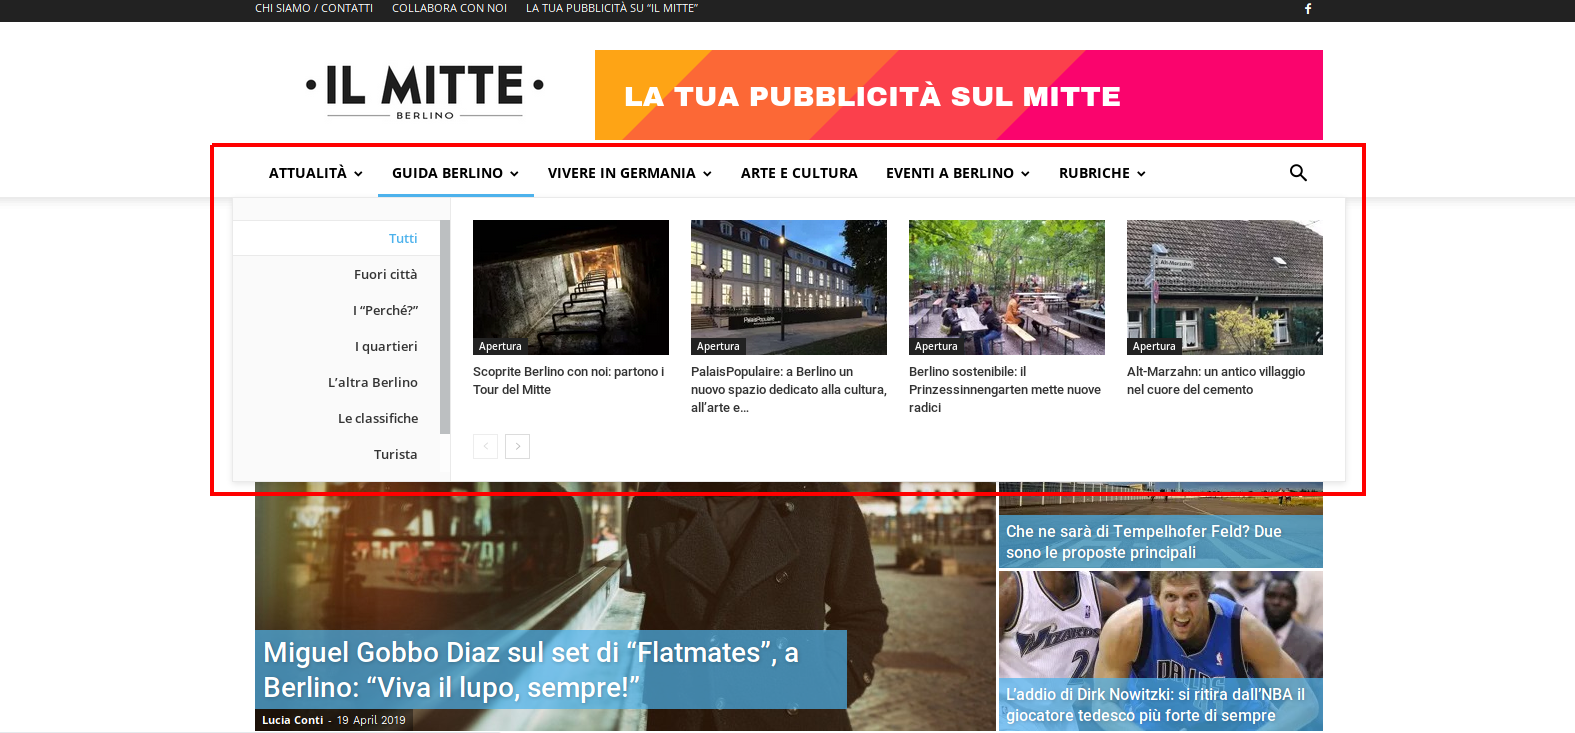
\includegraphics[width=35em]{img/menu}
\caption{Menù del sito}
\end{center}
\end{figure}
\vspace{30pt}

\paragraph*{Barra di ricerca}

Un primo problema di questo strumento di navigazione si evince dal primo sguardo: la barra non è direttamente visibile, bensì è necessario cliccare sulla lente d'ingrandimento per poterla aprire. \\
La barra d'inserimento permette la digitazione di 30 caratteri e mezzo (al trentunesimo scompare metà del primo carattere), quindi la lunghezza è sufficiente considerando la grandezza del sito. \\
La ricerca non è dinamica: per completare l'azione è necessario premere invio o cliccare sul pulsante "Cerca". 


\vspace{30pt}
\begin{figure}[htbp]
\begin{center}
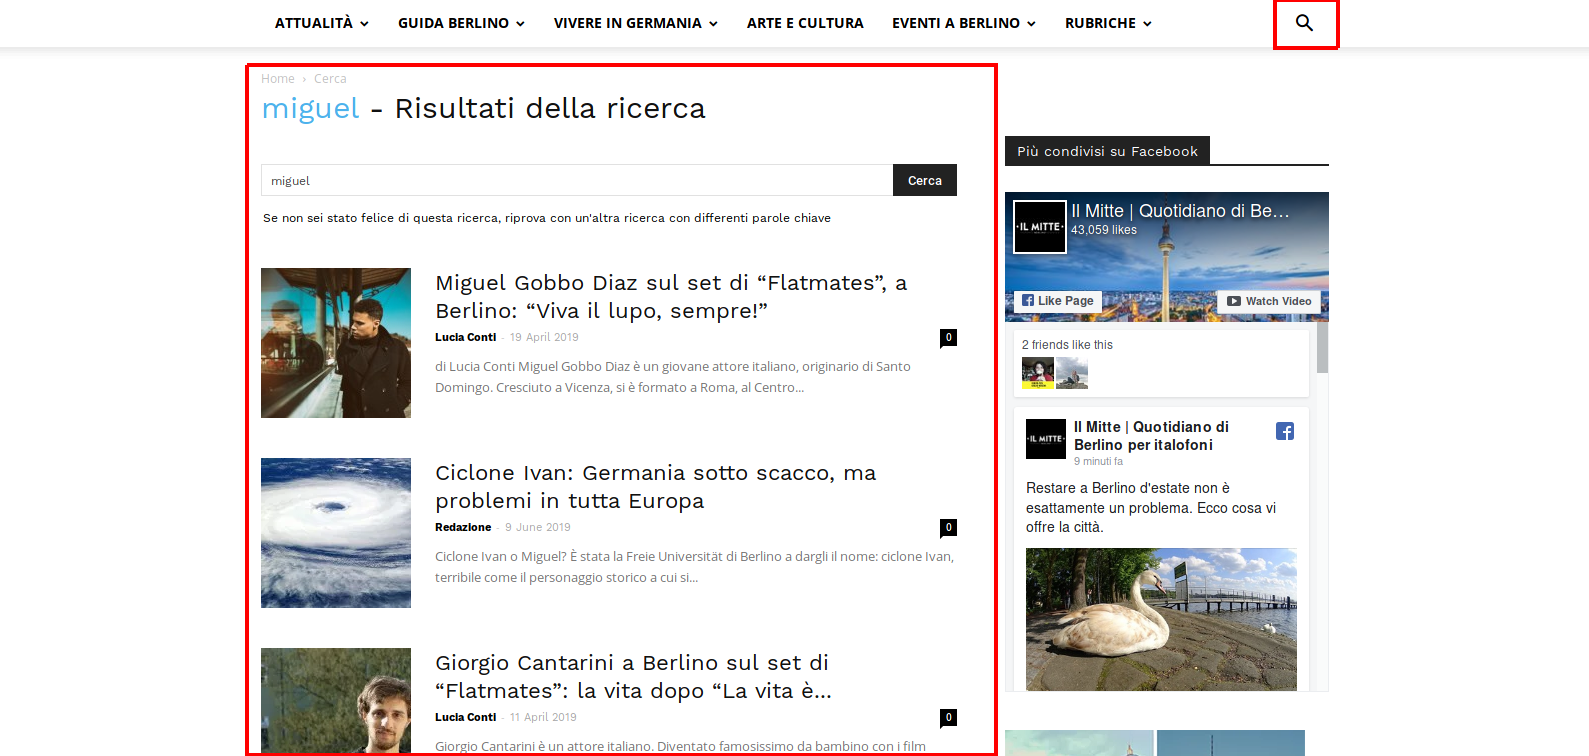
\includegraphics[width=35em]{img/ricerca}
\caption{Pulsante ricerca e risultato}
\end{center}
\end{figure}
\vspace{30pt}

\begin{figure}[htbp]
\begin{center}
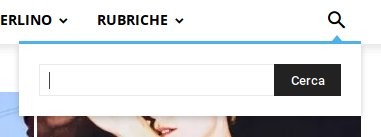
\includegraphics[width=25em]{img/barraricerca}
\caption{Barra di ricerca}
\end{center}
\end{figure}
\vspace{30pt}

La query richiede parecchio tempo per essere effettuata, con conseguente possibile spazientimento dell'utente. La ricerca comunque risulta accurata per le casistiche di test; l'ordine di visualizzazione è una combinazione di pertinenza e data di pubblicazione, e la modalità è a lista. Questo, insieme al numero di risultati limitato a nove, la rende adatta e funzionale.\\
Nel caso in cui la ricerca non vada a buon fine, la pagina visualizza solamente il messaggio "Nessun risultato per la tua ricerca"; questo è sufficiente, ma si poteva sicuramente implementare un altro sistema per ridurre la frustrazione dell'utente.